\documentclass[12pt]{article}

\usepackage[portuguese]{babel}

\usepackage{graphicx}
\usepackage[section]{placeins}
\usepackage{float}
\usepackage{url}

\graphicspath{ {figures} }

\addto\captionsportuguese{\renewcommand*\contentsname{Sumário}}

\author{João Vitor Maia Neves Cordeiro}
\title{Terceiro trabalho prático}
\date{\today}

\begin{document}

\maketitle

\clearpage

{\setlength\parskip{\fill}
    \tableofcontents
}


\section{Introdução}

Esse trabalho tem como objetivo estudar e aplicar na prática conceitos de gerência de redes através de uma ferramenta de monitoramento, utilizando os conhecimentos adquiridos em aula e em pesquisas externas para monitorar o tráfego de uma rede local, com ênfase na captura de pacotes dos protocolos TCP e HTTP. A ferramenta escolhida para realizar o trabalho é o Wireshark, por possuir filtros que facilitam a gerência, além de já se ter familiaridade com a ferramenta desde a confecção do segundo trabalho prático da disciplina.

O Wireshark é gratuito e nos permite monitorar, filtrar e identificar o tráfego de pacotes na rede onde está instalado. Além de possuir um formato próprio de arquivos que nos permite exportar as operações de monitoramento para serem carregadas em outras instâncias do programa.

\section{Funcionamento do protocolo}

\subsection{Começando a conexão}

Falando exclusivamente do protocolo TCP, o estabelecimento da conexão é feito com um processo chamado \emph{three-way-handshake} onde são enviadas 3 mensagens de sincronização em ambos os sentidos (ou seja, as duas partes da comunicação precisam estar sincronizadas). Durante esse processo, são trocadas informações importantes para o funcionamento da comunicação, como o \emph{checksum} de verificação, a timestamp e outros.

Os 3 passos são: primeiramente o cliente envia para o server um segmento com SYN (synchronization) com 0 bytes no campo de dados. O servidor então retorna com SYN/ACK, comunicando ao cliente que o pedido foi recebido. Ao receber isso, o cliente então finaliza o handshake enviando ACK afirmando que recebeu corretamente as informações enviadas pelo servidor.

\subsection{Finalizando a conexão}

O término da comunicação bem sucedida (que seguiu corretamente os passos do TCP) termina da seguinte forma: o cliente envia um segmento com a flag FIN, o servidor responde com um segmento de confirmação, perguntando se o cliente realmente deseja finalizar a conexão. Caso sim, o servidor envia uma mensagem com o segmento SYN/ACK para o cliente. Por fim, o cliente envia ACK para o servidor, finalizando a conexão.

\section{Desenvolvimento do experimento}

Como dito antes, foi utilizado o software Wireshark para o monitoramento da rede durante o experimento. Além disso, a flag inicial utilizada foi \emph{tcp} que serve para mostrar todos os pacotes que trafegam usando TCP. Essa é apenas a flag inicial e veremos depois que pode-se usar as flags mesmo ao final da captura para ajudar na interpretação dos resultados.

Optei por deixar apenas um website aberto durante o monitoramento para ter uma visualização melhor do passo a passo na comunicação entre duas fontes (o computador local e o servidor de aplicação que roda o website). O site utilizado foi o Youtube, que além de utilizar HTTPS (Protocolo TLS, Porta 433) para trafegar hipertexto, também usa o Websocket e outros protocolos para streaming de dados. Aqui iremos focar apenas na tranmissão HTTPS via TCP.

\subsection{Início da conexão TCP}

Ao acessar o website nós vamos iniciar também a comunicação, começando o processo do three-way-handshake. No caso abaixo os endereços IPs estão na versão 6. O cliente (2804:14d:baa1:b73e:a46e:d7ae:53f:1ad2) envia um SYN para o servidor (2800:3f0:4001:80f::200a) no pacote 53. O servidor responde com SYN/ACK no pacote 54 e por fim o cliente responde com ACK no pacote 55. Essa troca de mensagens pode ser vista na figura 1.

\begin{figure}[H]
    \centering
    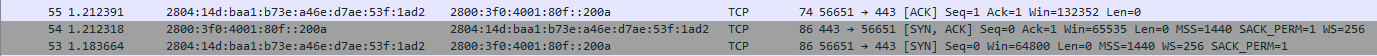
\includegraphics[width=\linewidth]{stablished.png}
    \caption{Estabelecimento de conexão.}
\end{figure}

\subsection{Transferindo dados}

Após ter a comunicação estabelecida pelo protocolo TCP, a tranmissão de dados pelas duas fontes pode ser realizada por diversos protocolos, aqui escolhi o popular HTTPS (Protocolo TLS, Porta 433), por ser o protocolo utilizado pelo Youtube e outras plataformas. O TLS em si possui uma camada de criptografia e um handshake separado além do que já foi realizado pelo TCP. Não irei cobrir essa criptografia e novo handshake nesse trabalho, mas o fluxo é parecido com o do TCP, apenas adicionando a criptografia ao meio com uma troca de chaves.

Após finalizados os procedimentos de segurança os dados podem ser trafegados no mesmo modelo do protocolo HTTP comum, com headers e um body, além de outros metadados. O TLS possui um keep-alive, então múltiplas tranmissões de dados podem ser realizadas a partir de um mesmo handshake. Na figura 2 podemos ver os pacotes que foram utilizados desde o início do handshake TLS até as transmissões de dados realizadas.

\begin{figure}[H]
    \centering
    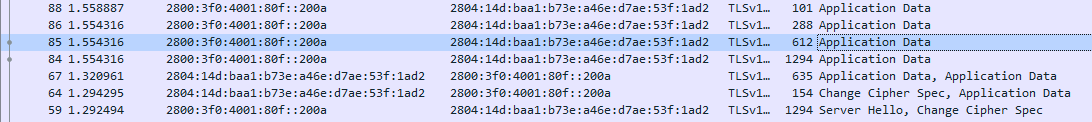
\includegraphics[width=\linewidth]{https_packages.png}
    \caption{Protocolo TLS transmitindo dados.}
\end{figure}

\subsection{Encerrando conexão TCP}

Como foi comentado antes, o final de uma conexão do protocolo TCP também possui uma espécie de "ritual". O cliente envia para o servidor uma mensagem com a flag FIN, o servidor então responde com FIN/ACK e o cliente confirma com ACK. Na figura 3 podemos ver isso acontecendo diversas vezes em conexões diferentes. Perceba o pacote 115 enviando um FIN/ACK que depois é respondido no 122 com ACK para finalizar completamente a conexão.

\begin{figure}[H]
    \centering
    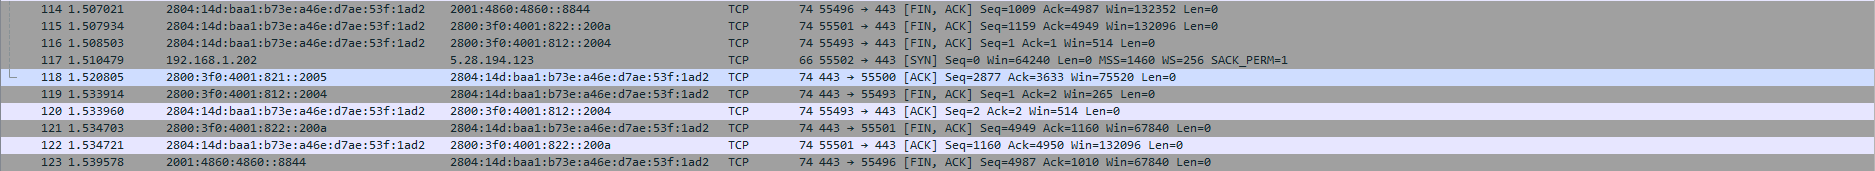
\includegraphics[width=\linewidth]{tcp_end.png}
    \caption{Finalizando conexão TCP.}
\end{figure}

\section{Conclusão}

Realizando esse trabalho foi possível perceber na prática o funcionamento de protocolos que fundamentam a rede mundial de computadores e a vida de todos nós. Ao analisar as entrelinhas do TCP e TLS podemos verificar o fluxo de dados que ocorre cada vez que abrimos um navegador ou fazemos uma requisição em um software externo. Além disso, durante o desenvolvimento do experimento pude ganhar mais conhecimento do software Wireshark, que se mostrou deverás útil no monitoramento de redes por possuir funcionalidades como filtragem e catalogação de conexões. Em suma, o trabalho cumpriu seus requisitos pedagógicos e didáticos para a formação de um profissional da ciência da computação.

\end{document}